\documentclass{article}
\usepackage[utf8]{inputenc}
\usepackage{listings} 
\usepackage{inconsolata} 
\usepackage{blindtext,expdlist} 
\usepackage{graphicx}
\graphicspath{ {./} }
\lstdefinelanguage{CISCO} 
{ 
sensitive=true, 
morekeywords=[1]{}, 
} 


\title{CO323 Lab 04}
\author{E/14/158\\Gihan Chanaka Jayatilaka }
\date{15/05/2018}

\begin{document}

\maketitle

\section{Design}
\subsection{File}
See E14158-CO323-Lab04.pkt\\
\subsection{Diagram}
\begin{figure}[h]
    \centering
    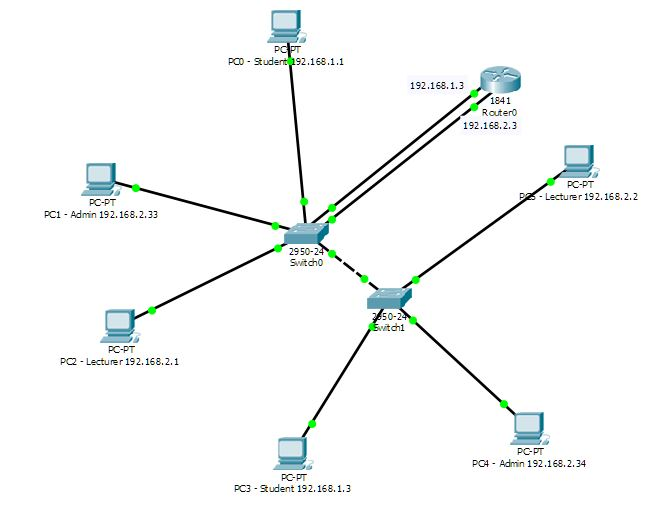
\includegraphics[scale=0.5]{VLANS}
    \caption{Network.jpg}
    \label{fig:Network configuration}
\end{figure}
\subsection{IP ranges}
\begin{table}[h]
    \centering
    \begin{tabular}{|l|c|c|c|}
         \hline
         Parameter&Students&Lecturers&Admin staff  \\
         \hline
         No of people&220&15&5\\
         IP bl0ck size&256&32&8\\
         IP range&192.168.1.0-192.168.1.255&192.168.2.0-192.168.2.31&192.168.2.32-192.168.2.39\\
         Subnet mask&255.255.255.0&255.255.255.224&255.255.255.248\\
         &192.168.1.0/24 & 192.168.2.0/27 & 192.168.2.32/29\\\
         
         Network IP&192.168.1.0&192.168.2.0&192.168.2.32\\
         Broadcast IP&192.168.1.255&192.168.2.31&192.168.2.39\\
         First IP for PC&192.168.1.1&192.168.2.1&192.168.2.33\\
         Last IP for PC&192.168.1.254&192.168.2.30&192.168.2.38\\
         IPs for PCs&254&30&6\\
         \hline
         PC IPs&192.168.1.1,2&192.168.2.1,2&192.168.1.33,34\\
         Router IP&192.168.1.3&192.168.2.3&\\
         
         \hline
    \end{tabular}
    \caption{Network}
    \label{tab:my_label}
\end{table}

\section{Commands}

\subsection{Switch 0}

\begin{lstlisting}[language=CISCO] 
Switch>enable
Switch#configure terminal 
Enter configuration commands, one per line.  End with CNTL/Z.
Switch(config)#interface fastEthernet 0/2
Switch(config-if)#switchport mode access
Switch(config-if)#switchport access vlan 2
Switch(config)#interface fastEthernet 0/3
Switch(config-if)#switchport mode access
Switch(config-if)#switchport access vlan 4
Switch(config)#interface fastEthernet 0/3
Switch(config-if)#switchport mode access
Switch(config-if)#switchport access vlan 3
Switch(config)#interface fastEthernet 0/1
Switch(config-if)#switchport mode trunk
Switch(config-if)#switchport nonegotiate
Switch(config-if)#switchport trunk allowed vlan 2-4
Switch#copy running-config startup-config

\end{lstlisting} 


\subsection{Switch 1}

\begin{lstlisting}[language=CISCO] 
Switch>enable
Switch#configure terminal 
Enter configuration commands, one per line.  End with CNTL/Z.
Switch(config)#interface fastEthernet 0/2
Switch(config-if)#switchport mode access
Switch(config-if)#switchport access vlan 3
Switch(config)#interface fastEthernet 0/3
Switch(config-if)#switchport mode access
Switch(config-if)#switchport access vlan 4
Switch(config)#interface fastEthernet 0/3
Switch(config-if)#switchport mode access
Switch(config-if)#switchport access vlan 2
Switch(config)#interface fastEthernet 0/1
Switch(config-if)#switchport mode trunk
Switch(config-if)#switchport nonegotiate
Switch(config-if)#switchport trunk allowed vlan 2-4
Switch#copy running-config startup-config

\end{lstlisting} 

\subsection{Router 0}

\begin{lstlisting}[language=CISCO] 
Router(config)#interface FastEthernet0/0
Router(config-if)#ip address 192.168.1.3 255.255.255.0
Router(config)#interface FastEthernet0/1
Router(config-if)#ip address 192.168.2.3 255.255.255.0
Router#copy running-config startup-config 
\end{lstlisting} 


\section{Ping and Tracert}

\subsection{Within student VLAN}
\textbf{\underline{From 192.168.1.1}}\\
\begin{lstlisting}[language=CISCO]
Pinging 192.168.1.2 with 32 bytes of data:

Reply from 192.168.1.2: bytes=32 time<1ms TTL=128
Reply from 192.168.1.2: bytes=32 time<1ms TTL=128
Reply from 192.168.1.2: bytes=32 time<1ms TTL=128
Reply from 192.168.1.2: bytes=32 time=15ms TTL=128

Ping statistics for 192.168.1.2:
    Packets: Sent = 4, Received = 4, Lost = 0 (0% loss),
Approximate round trip times in milli-seconds:
    Minimum = 0ms, Maximum = 15ms, Average = 3ms

C:\>tracert 192.168.1.2

Tracing route to 192.168.1.2 over a maximum of 30 hops: 

  1   0 ms      17 ms     0 ms      192.168.1.2

Trace complete.

C:\>ping 192.168.1.3

Pinging 192.168.1.3 with 32 bytes of data:

Reply from 192.168.1.3: bytes=32 time=143ms TTL=255
Reply from 192.168.1.3: bytes=32 time=1ms TTL=255
Reply from 192.168.1.3: bytes=32 time<1ms TTL=255
Reply from 192.168.1.3: bytes=32 time<1ms TTL=255

Ping statistics for 192.168.1.3:
    Packets: Sent = 4, Received = 4, Lost = 0 (0% loss),
Approximate round trip times in milli-seconds:
    Minimum = 0ms, Maximum = 143ms, Average = 36ms

C:\>tracert 192.168.1.3

Tracing route to 192.168.1.3 over a maximum of 30 hops: 

  1   0 ms      0 ms      0 ms      192.168.1.3

Trace complete.
\end{lstlisting}

\subsection{Within Lectuer VLAN}
\textbf{\underline{From 192.168.2.2}}\\
\begin{lstlisting}[language=CISCO]
C:\>ping 192.168.2.1

Pinging 192.168.2.1 with 32 bytes of data:

Reply from 192.168.2.1: bytes=32 time=1ms TTL=128
Reply from 192.168.2.1: bytes=32 time<1ms TTL=128
Reply from 192.168.2.1: bytes=32 time<1ms TTL=128
Reply from 192.168.2.1: bytes=32 time<1ms TTL=128

Ping statistics for 192.168.2.1:
    Packets: Sent = 4, Received = 4, Lost = 0 (0% loss),
Approximate round trip times in milli-seconds:
    Minimum = 0ms, Maximum = 1ms, Average = 0ms

C:\>tracert 192.168.2.1

Tracing route to 192.168.2.1 over a maximum of 30 hops: 

  1   0 ms      0 ms      0 ms      192.168.2.1

Trace complete.

C:\>ping 192.168.2.3

Pinging 192.168.2.3 with 32 bytes of data:

Reply from 192.168.2.3: bytes=32 time=20ms TTL=255
Reply from 192.168.2.3: bytes=32 time<1ms TTL=255
Reply from 192.168.2.3: bytes=32 time<1ms TTL=255
Reply from 192.168.2.3: bytes=32 time<1ms TTL=255

Ping statistics for 192.168.2.3:
    Packets: Sent = 4, Received = 4, Lost = 0 (0% loss),
Approximate round trip times in milli-seconds:
    Minimum = 0ms, Maximum = 20ms, Average = 5ms

C:\>tracert 192.168.2.3

Tracing route to 192.168.2.3 over a maximum of 30 hops: 

  1   0 ms      0 ms      0 ms      192.168.2.3

Trace complete.
\end{lstlisting}

\subsection{Within Admin VLAN}
\textbf{\underline{From 192.168.2.33}}\\
\begin{lstlisting}[language=CISCO]
C:\>ping 192.168.2.34

Pinging 192.168.2.34 with 32 bytes of data:

Reply from 192.168.2.34: bytes=32 time<1ms TTL=128
Reply from 192.168.2.34: bytes=32 time<1ms TTL=128
Reply from 192.168.2.34: bytes=32 time<1ms TTL=128
Reply from 192.168.2.34: bytes=32 time<1ms TTL=128

Ping statistics for 192.168.2.34:
    Packets: Sent = 4, Received = 4, Lost = 0 (0% loss),
Approximate round trip times in milli-seconds:
    Minimum = 0ms, Maximum = 0ms, Average = 0ms

C:\>tracert 192.168.2.34

Tracing route to 192.168.2.34 over a maximum of 30 hops: 

  1   1 ms      0 ms      0 ms      192.168.2.34

Trace complete.
\end{lstlisting}


\subsection{Between Student and Admin VLANs}
\textbf{\underline{From 192.168.1.1}}\\
\begin{lstlisting}[language=CISCO]
C:\>ping 192.168.3.33

Pinging 192.168.3.33 with 32 bytes of data:

Reply from 192.168.1.3: Destination host unreachable.
Reply from 192.168.1.3: Destination host unreachable.
Reply from 192.168.1.3: Destination host unreachable.
Reply from 192.168.1.3: Destination host unreachable.

Ping statistics for 192.168.3.33:
    Packets: Sent = 4, Received = 0, Lost = 4 (100% loss),
\end{lstlisting}


\subsection{Between Student and Lecturer VLANs}
\textbf{\underline{From 192.168.1.1}}\\
\begin{lstlisting}[language=CISCO]
C:\>ping 192.168.2.1

Pinging 192.168.2.1 with 32 bytes of data:

Request timed out.
Reply from 192.168.2.1: bytes=32 time<1ms TTL=127
Reply from 192.168.2.1: bytes=32 time<1ms TTL=127
Reply from 192.168.2.1: bytes=32 time<1ms TTL=127

Ping statistics for 192.168.2.1:
    Packets: Sent = 4, Received = 3, Lost = 1 (25% loss),
Approximate round trip times in milli-seconds:
    Minimum = 0ms, Maximum = 0ms, Average = 0ms

C:\>tracert 192.168.2.1

Tracing route to 192.168.2.1 over a maximum of 30 hops: 

  1   0 ms      0 ms      0 ms      192.168.1.3
  2   0 ms      0 ms      0 ms      192.168.2.1

Trace complete.
\end{lstlisting}


\section{Conclusion}
\begin{itemize}
    \item The switches are transparent. The devices within a particular VLAN can directly send a packet to the other devices. \\
    \item Even when the devices are in the same switch, they cannot communicate unless they are on the same VLAN (in absence of other mechanisms).\\
    \item If two devices are on same switch, different VLANS they can communicate using a layer 3 packet forwarding device. eg: Router or L3 switch.\\
    \item Even when the devices are connected to the same switch, if they are on different VLANs connected by a router, the packets need additional hops. (The switch is not transparent across VLANS.\\
\end{itemize}





\end{document}
